\section{Performance Evaluation}

Eine Audio-Plugin läuft in einer Umgebung mit vielen anderen Komponenten mit dem es CPU-Ressourcen teilt. Die Verarbeitung von Audiodaten muss innerhalb diskreten, von der Audio-Hardware gesteuerten, Zeitintervallen abgeschlossen werden. Typische Audio-Sampling-Frequenzen sind 44,1 kHz, 48 kHz, 88,2 kHz und 96 kHz. Mit 44,1 kHz als Beispiel bedeutet dies, daß die für eine einzelne Abtastung erforderlichen Berechnungen innerhalb von 0,023 ms durchgeführt werden muss. Interrupts müssten von der Audio-Hardware in Abständen von 0.023ms getätigt werden, und dies würde das Betriebssystem der CPU überlasten. Stattdessen werden Anfragen für neue Audiodaten in Puffern gebündelt. Die Größe der Puffer ist ein Parameter, der vom Benutzer gestzt werden kann. In der Regel beträgt es 512 Abtastungen, kann aber bis 16 Abtastungen klein sein.

Erhöht man der Puffergröße steigt auch die Zeit, die die CPU hat, um die Audiodaten zu verarbeiten. Dies führt aber auch dazu das  die Latenz das System steigt. Eine Puffergröße von 512 Abtastungen entspricht einer Latenzzeit von 11.60ms. Ein 16-Probenpuffer Größe entspricht 0.36ms.

Braucht ein einzelnes Plugin 1,0 ms auf seine Verarbeitung abzushliessen, dann wird es nicht rechtzeigtig beendet, wenn die Puffergröße zu niedrig eingestellt ist. Wenn die Puffergröße gerade hoch genug ist, dann bleibe nicht genügend CPU-Ressourcen übrig für andere Plugins, ihre Berechnungen zu auszuführen.

\subsection{Synchronous Performance}

Dieses Projekt verteilt die Verarbeitung an externen SBC-Geräte. Es gibt jedoch keine Entlastung , wenn die Audio-Plugin blockiert ist, während es für die Ergebnisse aus dem SBC-Gerät wartet. Da die externe SBC-Geräte langsamer sind als der Haupt-CPU wird die Bearbeitungszeit sogar länger. Fügt man der Zeit hinzu, die zur Serialisierung und Deserialisierung das Datagramm-Paket an jedem Ende benötigt wird, wird die Leistung sogar noch verschlechtern.

Abbildung~\ref{fig:local_vs_remote} zeigt das Problem genauer.

\begin{figure}[H]
    \centering
    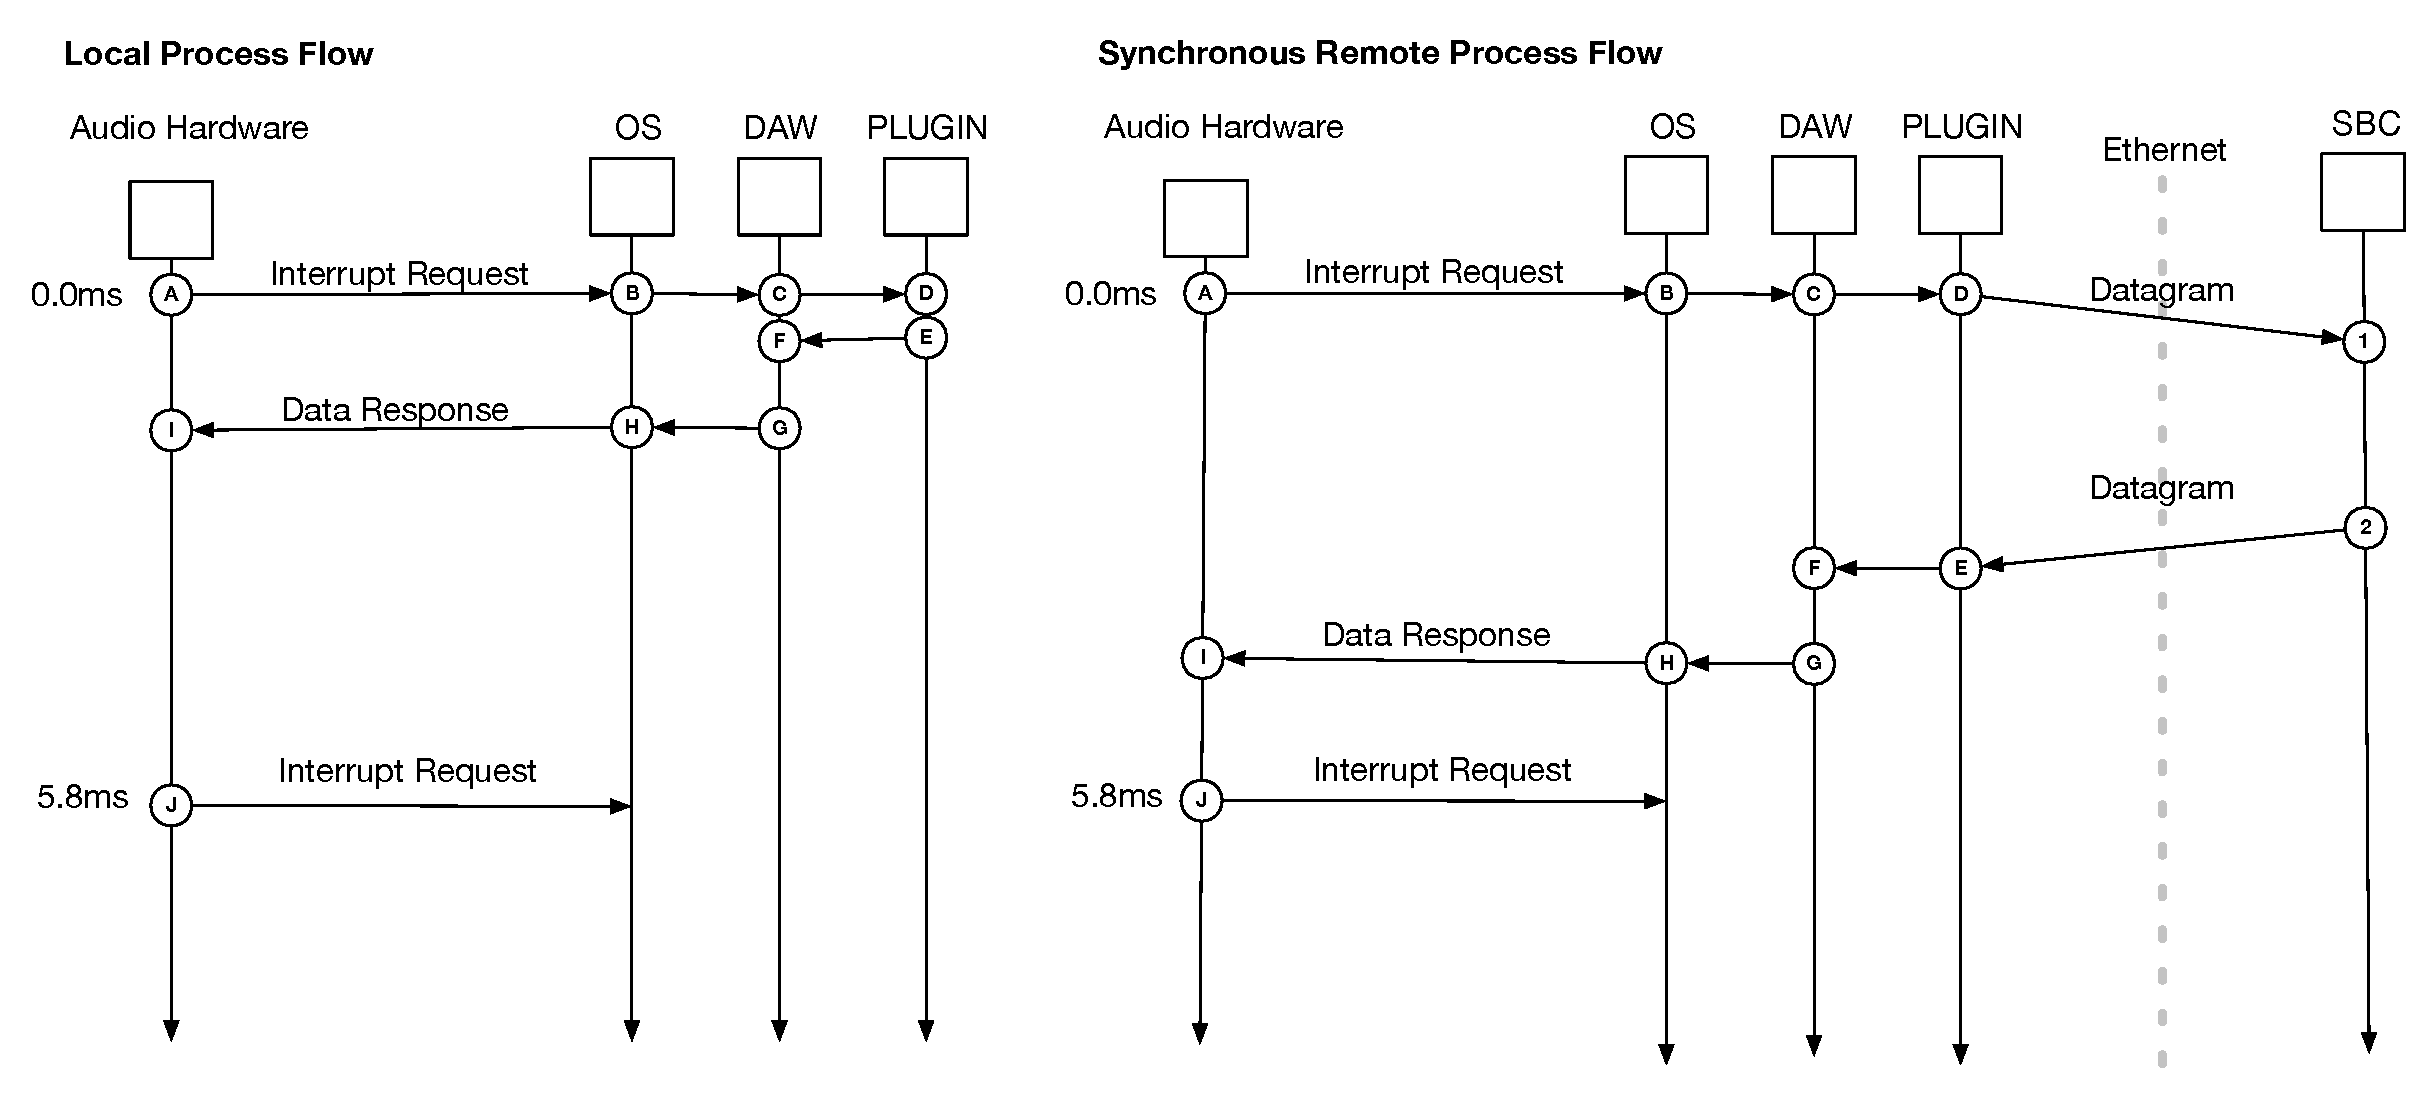
\includegraphics[width=\textwidth]{assets/conclusion/process_flow_compared.pdf}
    \caption{Local vs Remote Synchronous Processing}
    \label{fig:local_vs_remote}
\end{figure}

Das Beispiel zeigt die Audio-Hardware Abfragen an das Betriebssystems, in Zeitintervallen von 5,8 ms getacktet. Dies entspricht einer Puffergröße von 256 Abtastwerten. Das Zeitintervall zwischen den Staaten D und E repräsentiert die Zeit, die ein Plugin braucht, um einen Puffer von 256 Proben zu verarbeiten. Die DAW-Anwendung führt andere notwendige Audio-Verarbeitungsfunktionen in dem Intervall zwischen F und G. Nach Zustände G und H sind der DAW-Anweung und Betriebssystems wieder in der Lage andere Dinge zu tun, wie z.B. die GUI zu aktualisieren.

Mit der synchronen verteilte Verarbeitung wird der Zustand E blockiert bis Zuständen 1 und 2 abgeschlossen sind. Wenn diese Zeit signifikant ist dann hindert dies die DAW-Anwendung und Betriebssystem andere wichtige Aufgaben durchzuführen.

\begin{table}[H]
\begin{center}
\begin{tabular}{ |p{1.4cm}||p{1.5cm}|p{1.7cm}|p{1.7cm}|p{1.6cm}|p{1.4cm}|  }
 \hline
 puffergrösse    & pufferzeit (ms)    & rtTime (ms)   & pTime (ms)    & tTime (ms) & \% von pufferzeit\\
 \hline
 64             & 1.451247      & 0.574672          & 0.015857          & 0.558815      & 39.59 \\
 96             & 2.176870      & 0.575419          & 0.015851          & 0.559568      & 26.43 \\
 128            & 2.902494      & 0.59001           & 0.016519          & 0.573491      & 20.32 \\
 192            & 4.353741      & 0.67902           & 0.019013          & 0.660007      & 15.59 \\
 256            & 5.804988      & 0.707267          & 0.020352          & 0.686915      & 12.18 \\
 512            & 11.60997      & 0.707905          & 0.026348          & 0.681557      & 6.097 \\
 \hline
\end{tabular}
\end{center}
\caption{Measured Times for Synchronous Processing}
\label{tab:latency_comp}
\end{table}

Tabelle~\ref{tab:latency_comp} zeigt die gemessenen Zeiten für verschiedene Puffergrößen in der synchrone Ausführung, in der keine tatsächlich Audioverarbeitung statfindet. Nur die Vorbereitungs- und Tranport-Zeiten werden berücksichtigt. Ein Audiosystem läuft mit einer Puffergröße von 64 Proben hat 1.451ms, um alle Aufgaben zu erledigen. "rtTime" ist die gemessene Gesamtumlaufzeit. Dies entspricht der Zeit zwischen den Staaten D und E des synchronen Verfahrens in Abbildung~\ref{fig:local_vs_remote}. "pTime" ist Zeitintervall zwischen den Zuständen 1 und 2 auf der SBC-Gerät, den Zeitaufwand für die Verarbeitung der Daten. In diesem Fall gab es keine Verarbeitung, so ist dies nur die Zeitaufwand für die Deserialisierung und Serialisierung der Datagramme zu Audio- und MIDI-Daten. "tTime" ist der "ptime" subtrahiert von der "rtTime" welche das Verpackungsaufwand entspricht, um Daten zu senden und empfangen.

Die letzte Spalte, "\% of limit", zeigt wieviel Zeit insgesamt als prozentualer Anteil der "limit" verbraucht wurde. Bei einer Puffergröße von 64 Abtastungen wird 39.59 \% Prozent der Gesamtzeit für einer einzigen Plugin verbraucht. Es bleibt nicht viel Zeit übrig für andere Prozesse auf der CPU. Für eine Puffergröße von 512 Samples ist der "\% der Grenze" Wert viel niedriger. Dafür ist aber die Gesamtsystemlatenz geringfügig höher als die angestrebten maximal von 10ms. Durch das synchrone implementation wird die Verarbeitungslast der CPU überhaupt nicht verringert .


\subsection{Asynchronous Performance}

Anstatt auf eine Antwort von dem SBC zu Warten wie im obigen synchrone Methode, prüfft die asynchrone Methode ob Daten vorhanden sind. Falls Daten vorhanden sind, gibt es diese zurück, falls nicht gibt es leere Daten zurück. Die erste Anfrage für Audiodaten würde leere Daten zurück geben, aber in der Zeit bis zweite Puffer angefordert wird, kommt die erste Antwort von der SBC-Gerät zurückgekehrt. In beiden Fällen ist die einzige Zeit, die der Audio-Plugin selbst verbraucht, ist die Zeit das es braucht, für die Serialisierung, Deserialisierung, und Transport der Daten. Das sind die Abstände zwischen den Zuständen D und E und M und N dargestellt in Abbildung~\ref{fig:async_remote}.

\begin{figure}[H]
    \centering
    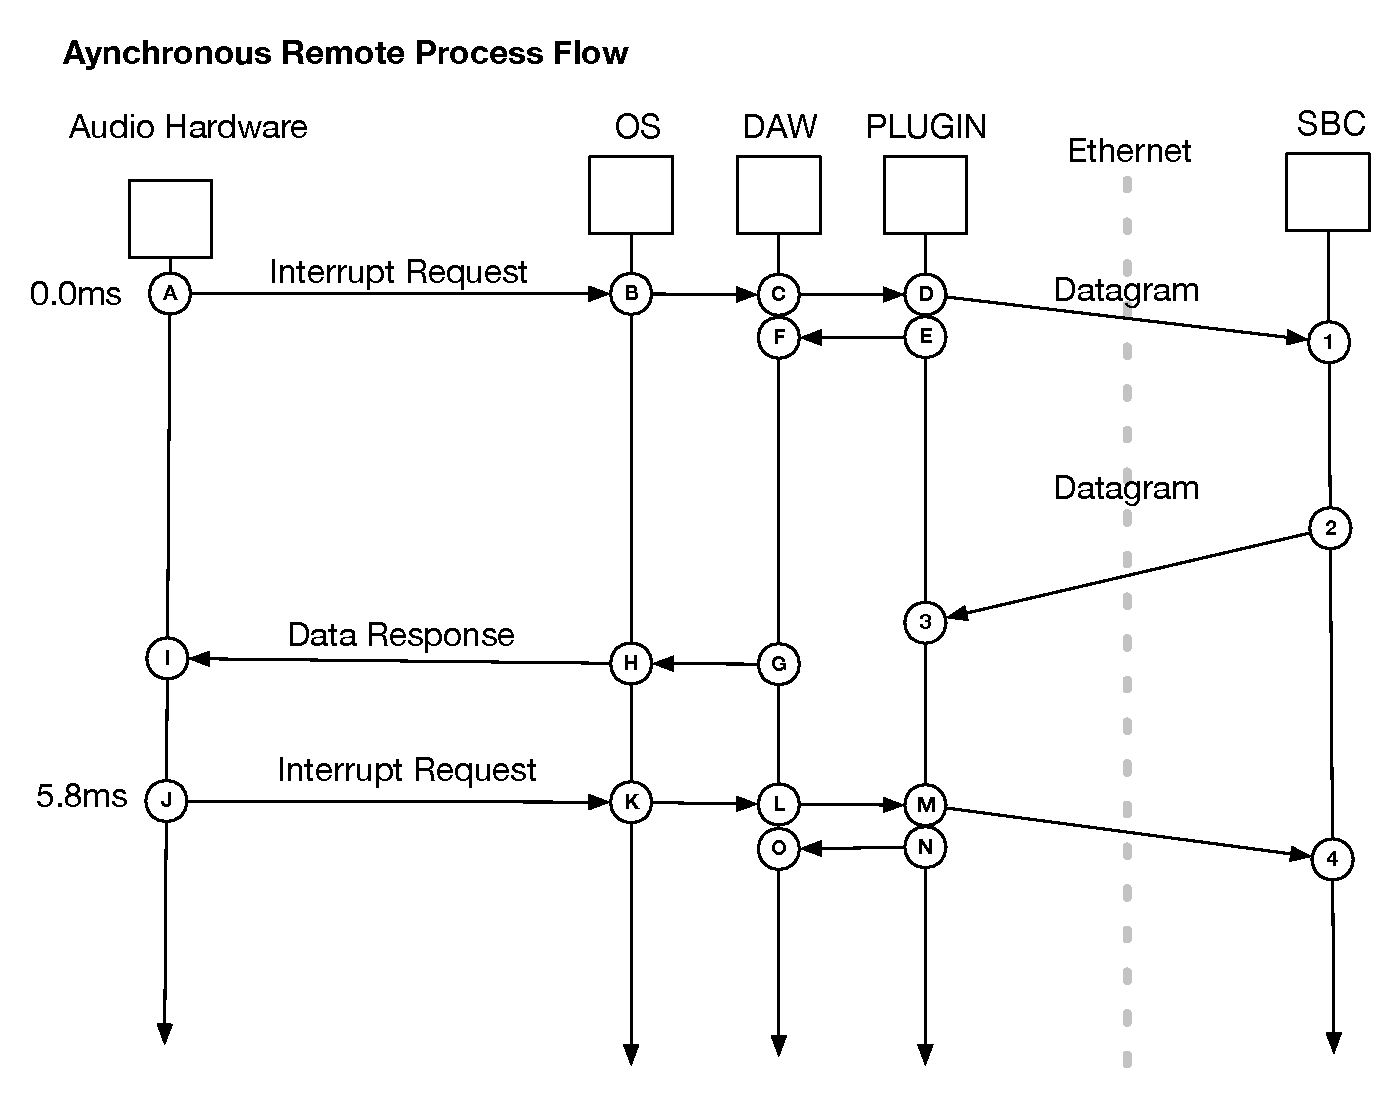
\includegraphics[width=\textwidth]{assets/conclusion/async_flow.pdf}
    \caption{Local vs Remote Synchronous Processing}
    \label{fig:async_remote}
\end{figure}

Bis der zweite Zyklus beginnt (J in Abbildung~\ref{fig:async_remote}), sind die verarbeiteten Daten aus dem ersten Zyklus zurückgekehrt. Die Zeit zwischen den Ereignissen M und N ist nicht mehr proportional zur Zeit benötigt, um tatsächlich die Daten zu verarbeiten, sondern um die Zeit, für das Senden und Empfangen der Daten. Tabelle B zeigt die gemessenen Zeiten.

\begin{table}[H]
\begin{center}
\begin{tabular}{ |p{1.4cm}||p{1.5cm}|p{1.7cm}|p{1.7cm}|p{1.6cm}|p{1.4cm}|  }
 \hline
 puffergrösse    & pufferzeit (ms)    & rtTime (ms)   & pTime (ms)    & tTime (ms) & \% von pufferzeit\\
 \hline
 64             & 1.451247      & 0.031683          & 0.015633          & 0.016050      & 2.18 \\
 96             & 2.176870      & 0.046585          & 0.016076          & 0.030509      & 2.14 \\
 128            & 2.902494      & 0.034745          & 0.016712          & 0.018032      & 1.19 \\
 192            & 4.353741      & 0.052279          & 0.018800          & 0.033478      & 1.20 \\
 256            & 5.804988      & 0.065752          & 0.019646          & 0.046105      & 1.13 \\
 512            & 11.60997      & 0.062939          & 0.019708          & 0.043230      & 0.54 \\
 \hline
\end{tabular}
\end{center}
\caption{Für asynchrone Datenverarbeitung gemessene Zeiten}
\label{tab:latency_async}
\end{table}



In der obigen Tabelle entspricht "rtTime" nicht mehr der tatsächlichen Gesamtverarbeitungszeit. Da die Daten zum Zeitpunkt der Interrupt bereits vorhanden sind, kann das Plugin diese Daten sofort zurückzugeben. Dies geht auf Kosten der Latenzzeit welche jetzt genau einer Interrupt-Zyklus entspricht. Der Benutzer kann die Puffergröße des Audiosystems einstellen, dass dies weit unter der 10 ms Grenze ist, ohne dass mehr als 1,2 \% der Bearbeitungszeit verwendet wird.

Die asynchrone Verfahren bringt einen echten Nutzen für die verteilte Verarbeitung in Bezug auf der Belastung der CPU. Der Preis ist jedoch eine Erhöhung der Latenzzeit des Plugins. Die verarbeiteten Audiodaten sind immer einen Puffer-Zyklus verzögert. Ein weiterer Nachteil ist, dass, wenn mehrere verteilte Prozessoren sind in einer Reihe verkettet sind, wie es in der Demo-Anwendung der Fall ist, dann ist die Latenzzeit ist kumulativ. Dies resultiert in einer Gesamtlatenz, der die "limit"-Zeit multipliziert mit der Anzahl der Prozessoren im Plugin gleich ist.

\subsection{Mögliche Optimierungen}

Es gibt zwei Bereiche, wo unnötige Operationen durchgeführt werden und optimiert werden könnten. Die erste ist die Serialisierung und Deserialisierung von Daten, wenn sie von der SBC-Gerät zurückgegeben werden. Sind in der Plug-in mehrere Prozesse nacheinander verkettet, wird der zurück  geschickte DiauproMessage zwischen jeder Prozess-Schritt unnötig deserialisiet und reserialisiert. Dies wäre eine relativ einfache Optimierung zu implementieren.

Die zweite Optimierung ist ähnlich, aber komplizierter zu implementieren. In einer Kette, nacheinandergeschalteten Prozessen müssten die Daten nicht nach jedem Schritt an das Master Plug-in zurückgeschickt werden, sondern direkt an den nächsten Knoten. Wenn der nächste Knoten auf dem gleichen SBC-Geräts befindet wird eine zusätzliche schritt über Ethernet ersparrt. Außerdem könnte auch die Serialisierungs Schritten zwischen den Knoten übersprungen werden, wenn die Knoten ihre Berechnungen direkt auf die Daten in dem DiauproMessage ausführen. Hierzu müsste die DiauproMessage erweitert werden, um Routing-Informationen zu erfassen, so dass jeder Rechennoten weiß, wo die Daten als nächstes geschickt werden müssen.

Obwohl komplexer, die zweite Optimierung hat den zusätzlichen Vorteil, dass die Latenzzeit sich nicht um ein Vielfaches der vollen Zykluszeit zwischen Interrupt-Aufrufe multipliziert wird. Die endgültigen Daten könnten nach einem einzigen Interrupt-Zyklus zurück gegeben werden.


